\section{Búsqueda de vacantes de oxígeno en SrTiO$_3$ mediante imágenes 4D-STEM}

% Introducción con información física sobre las vacantes de oxígeno en STO y cómo están ligadas a las propiedades del material. ¿Para qué se usa STO?

Los óxidos con estructura de perovskita son materiales complejos que se caracterizan por presentar una gran variedad de propiedades físicas muy interesantes. En nuestro caso hablaremos del SrTiO$_3$ (STO), un material dieléctrico que a 300 K presenta un gap de 3.2 eV.\\

El STO es una perovskita muy sensible al dopado, pues sus propiedades físicas se pueden ver alteradas drásticamente ante pequeños cambios en su composición. Concretamente, si sobre un sustrato de STO con una pequeña concentración de vacantes de oxígeno se hace crecer una fina capa de LaAlO$_3$ (LAO, otra perovskita dieléctrica), se ha podido medir experimentalmente que en la interfase aparece una alta conductividad eléctrica \cite{STO}. Este fenómeno se debe a la estabilización del gas bidimensional electrones bidimensional que vive en la intercara.

\subsection{Procesamiento de imágenes ABF de SrTiO$_3$}

En esta sección nos dedicaremos al análisis de datos experimentales rutinarios obtenidos en el Centro Nacional de Microscopía Electrónica de la UCM. Contamos con una muestra de STO cuya concentración de vacantes de oxígeno es desconocida, nosotros trataremos de ayudar caracterizarla.\\

\begin{wrapfigure}{o}{5.5cm}
    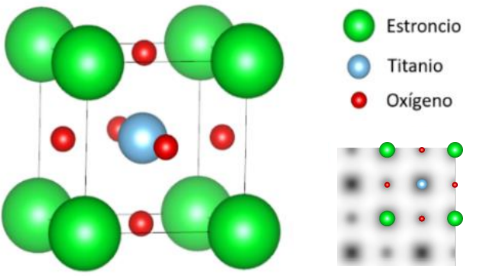
\includegraphics[width=0.34\textwidth]{fig/Fig15.png}
    \caption{En esta imagen se muestra un esquema de la celda unidad de SrTiO$_3$ (STO), junto a su visualización sobre una imagen simulada ABF \cite{paquito}.}
    \label{fig:15}
\end{wrapfigure} 

La muestra STO de la \autoref{fig:16} se está utilizando para diseñar nuevos detectores basados en 4D-STEM capaces de resolver entre columnas de oxígeno con y sin vacantes. No obstante, los datos que se han tomado en una primera sesión de STEM tienen tal cantidad de ruido que dichas columnas de oxígeno resultan indistinguibles a simple vista.\\

Partiendo de la imagen ABF que se muestra en la Figura \ref{fig:16}a, llevaremos a cabo varios procesos de \textit{denoising}. Nuestro objetivo principal es sacar a la luz esas columnas de oxígeno que, según se muestra en la simulación de la \autoref{fig:15}, deberían de poder apreciarse sin problemas sobre la región de integración del patrón de difracción en la que estamos trabajando.

\begin{figure}[h!]
    \centering
    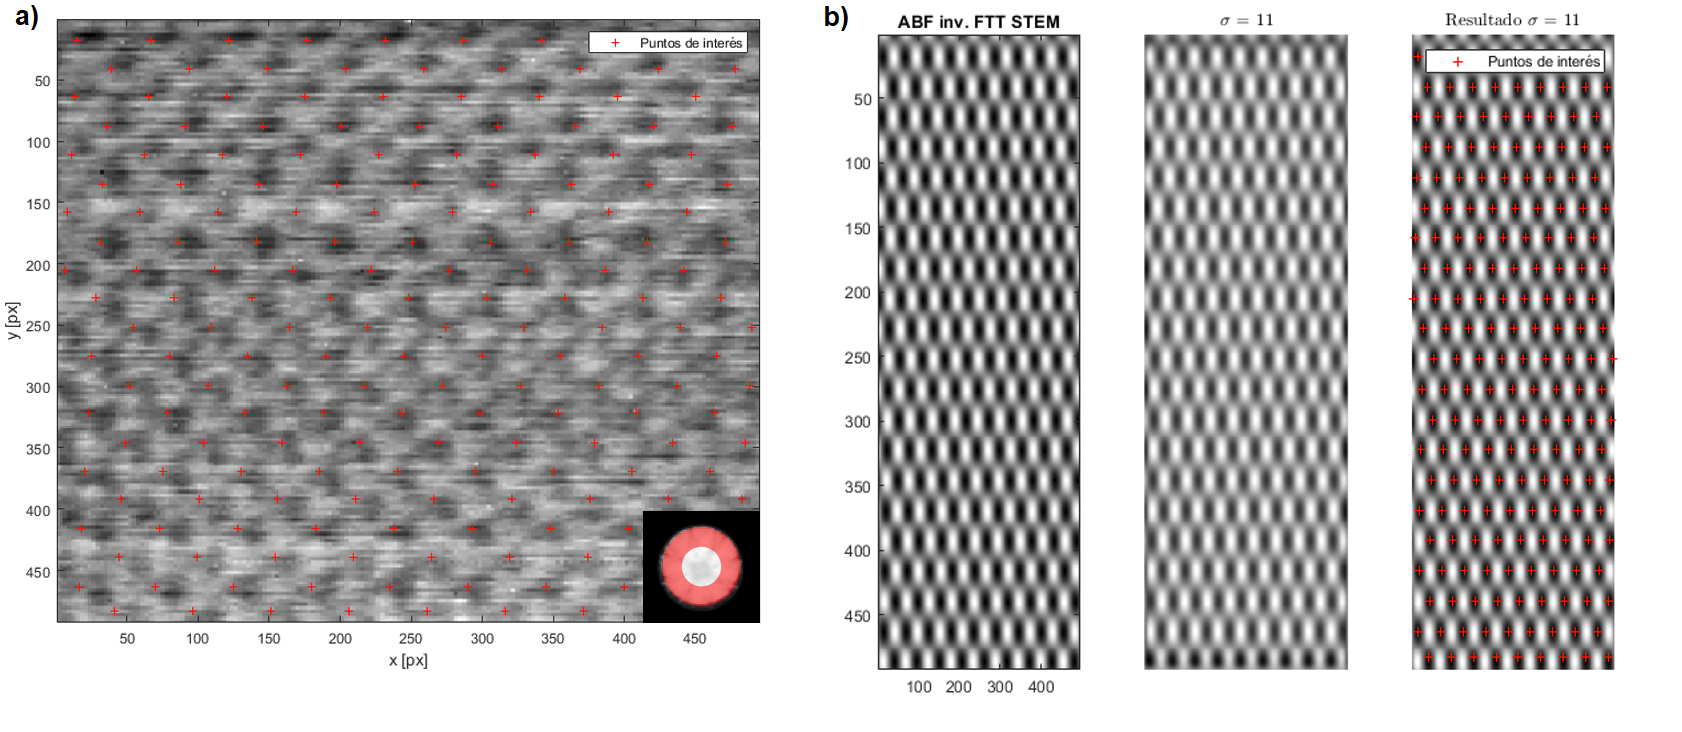
\includegraphics[width=1\textwidth]{fig/Fig16.png}
    \caption{\textbf{a)} Imagen ABF tomada por Francisco Fernández Cañizares (Departamento de Física de Materiales, UCM) sobre una muestra de STO horneada a 500 ºC durante 8 h - 6C 10cm df0. En la esquina inferior derecha aparece la región de integración sobre el patrón de difracción (15:30 mrads) seleccionada para generar dicha imagen. Los puntos de interés han sido escogidos por el algoritmo de detección de \textit{blobs}, cuyo \textit{input} corresponde con \textbf{b)} un filtrado FFT de alto umbral sobre la imagen ABF invertida. Programa desarrollado en MATLAB por el autor \cite{repo}.}
    \label{fig:16}
\end{figure}

\subsubsection{Generación de parches con información sobre la celda unidad}

La entrada para los distintos algoritmos de \textit{denoising} será un \textit{stack} de parches (ver Figura \ref{fig:17}a) que únicamente van a contener información sobre la celda unidad STO. Para llevar a cabo esta selección, inicialmente aplicaremos un PCA a los parches generados entorno a todos los puntos de interés. Esto nos permitirá filtrar en función de la primera componente principal aquellos parches que corresponden a columnas de Ti.\\

\subsubsection{\textit{Denoising} por PCA y NMF}

Una vez hemos generado el \textit{clean stack} de celdas unidad, volvemos a aplicar PCA y NMF (Figura \ref{fig:17}c), esta vez para realizar un promedio que nos permita extraer la información común entre todas las imágenes del \textit{stack}.

\subsubsection{\textit{Denoising} por una red neuronal con topología de \textit{autoencoder}}

Un \textit{autoencoder} es un tipo de red neuronal que se va a encargar de codificar las características más críticas de un \textit{dataset} mediante \textbf{aprendizaje no supervisado}. La simetría en la topología de este tipo de redes es fundamental, en nuestro caso seleccionaremos $m^2$-5-5-5-5-$m^2$, donde $m^2$ corresponde con el número de píxeles presentes en cada parche.\\

Si lo que buscamos es utilizar un \textit{autoencoder} para reducir el ruido de una imagen, el primer paso es añadir a nuestro \textit{clean stack} un ruido gaussiano de forma artificial. De este modo, generaremos el \textit{noisy stack} que se muestra en la Figura \ref{fig:17}a, el \textit{input} de nuestra red. Una vez contamos con esta entrada, entrenaremos al \textit{autoencoder} imponiendo que su salida sea similar a las imágenes contenidas en el \textit{clean stack}. Así, tras 300 iteraciones, obtenemos el resultado que se muestra en la Figura \ref{fig:17}b.

\newpage
\begin{figure}[h!]
    \centering
    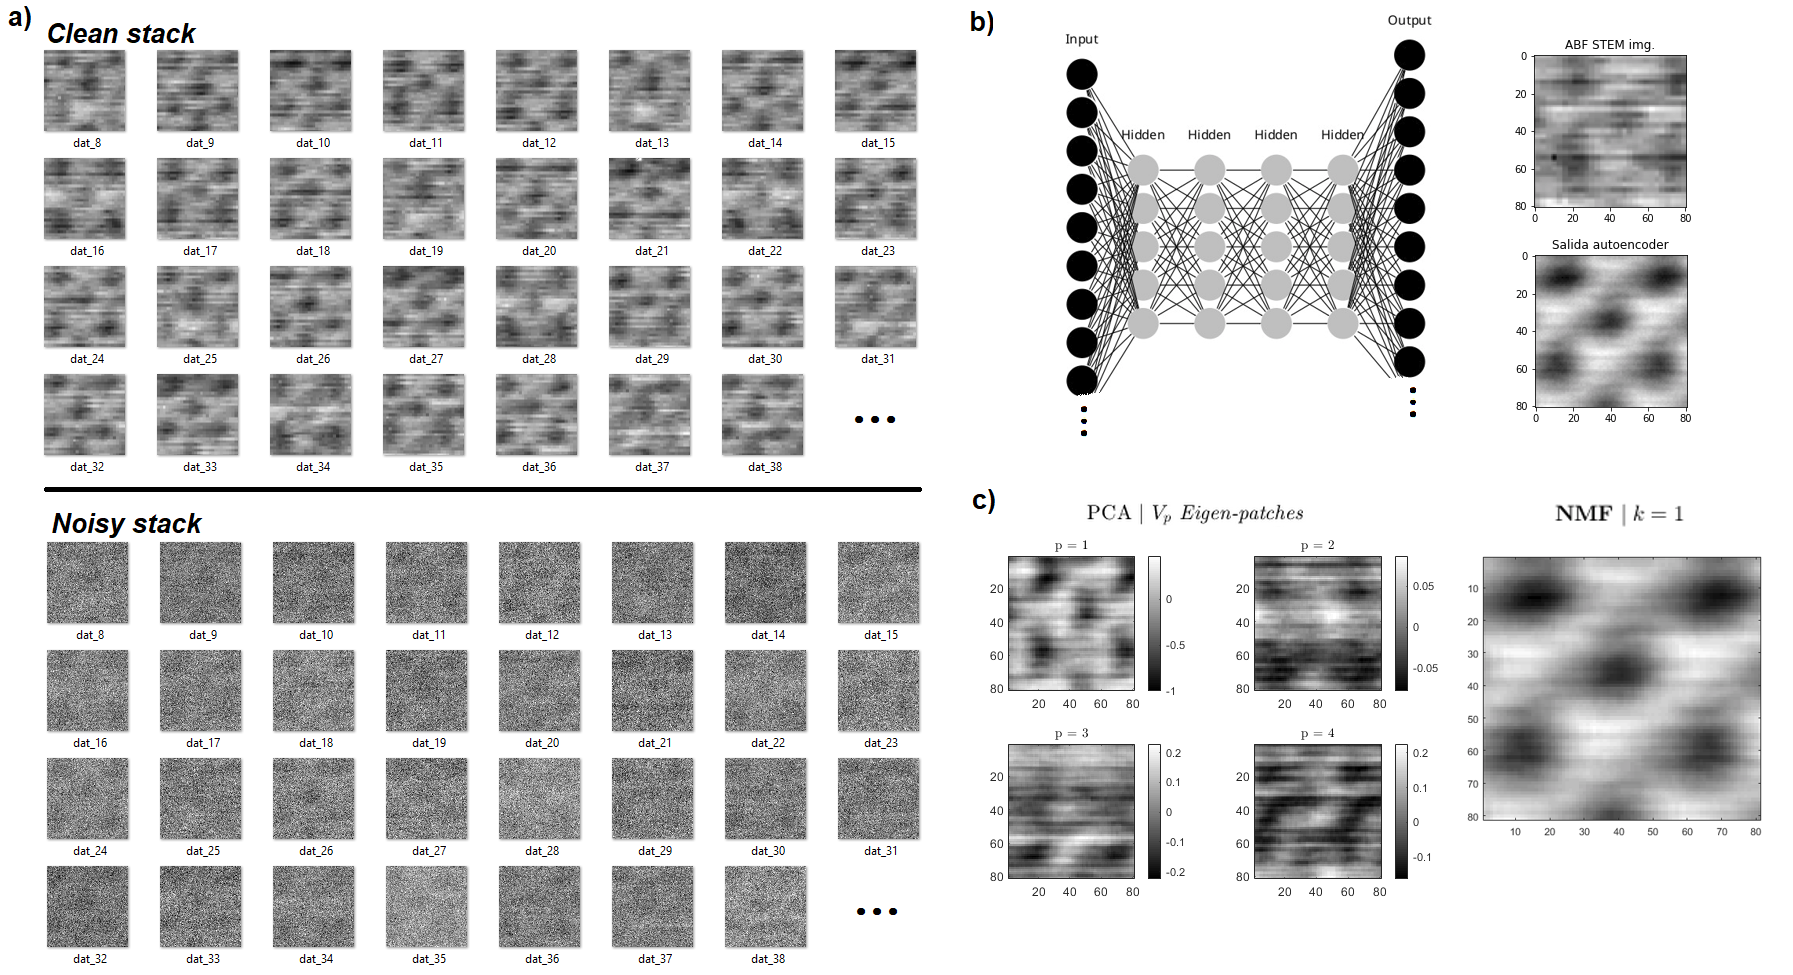
\includegraphics[width=1\textwidth]{fig/Fig17.png}
    \caption{ Figura que muestra \textbf{a)} algunos de los parches contenidos en cada \textit{stack}, \textbf{b)} la topología del \textit{autoencoder} junto a su salida tras un entrenamiento de 300 iteraciones a un \textit{learning rate} de 0.2, y \textbf{c)} el resultado de aplicar PCA y NMF sobre el \textit{clean stack}. Todo el código escrito por el autor en relación a este análisis se encuentra en el capítulo 4 de la referencia \cite{repo}.}
    \label{fig:17}
\end{figure}

\subsection{Análisis de resultados}

La alta definición de las columnas de Ti y Sr en la \autoref{fig:17} muestra claramente cómo es posible entrenar con éxito a la red neuronal para localizar los detalles deseados. En este caso, el resultado nos sirve para concluir que en nuestra imagen ABF no contamos con suficiente información sobre las columnas de oxígeno como para poder caracterizarlas. Este ejemplo demuestra cómo los algoritmos basados en técnicas de IA pueden tener éxito en localizar comportamientos en el ruido, aunque para ello necesitamos grandes volúmenes de datos que nos permitan mejorar la estadística del sistema, haciendo más relevante aquella información que queda diluida entre el ruido.

\addcontentsline{toc}{section}{Conclusiones} \normalsize
\section*{Conclusiones}

A lo largo de este trabajo hemos revisado el estado del arte en la aplicación de técnicas estadísticas y de IA a microscopía electrónica multidimensional, desarrollando una serie de algoritmos que hemos conseguido aplicar con gran éxito a datos de STEM rutinarios. Dicho logro, nos permite concluir este trabajo con una visión muy positiva en cuanto al futuro de este tipo de técnicas como una herramienta fundamental de caracterización, capaz de apoyar al científico en el estudio y descubrimiento de nuevos materiales avanzados.